%%%%%%%%%%%%%%%%%%%%%%%%%%%%%%%%%%%%%%%%%%%%%%%%%%%%%%%%%%%%%%%%%%%%%%
% Lớp 10 | Bất phương trình bậc 2 một ẩn | Dấu của tam thức bậc 2
% Dạng 0D7?1-2: Dấu của tam thức bậc 2 và ứng dụng
% Số câu: 38  (sinh tự động bởi tach_cau.py; từ nay thầy sửa trực tiếp file này)
%%%%%%%%%%%%%%%%%%%%%%%%%%%%%%%%%%%%%%%%%%%%%%%%%%%%%%%%%%%%%%%%%%%%%%

%%%%%%%%%%%%%%%% TRẮC NGHIỆM 4 PHƯƠNG ÁN %%%%%%%%%%%%%%%%

% nguồn: MaHoaNH_TracNghiem_Lop10
\begin{ex}%[0D7N1-2]%[ma:31e2c234]
	Cho tam thức $f(x)=a x^2+bx+c  ~(a \neq 0)$, $f(x)<0$, $\forall x \in \mathbb{R}$ khi và chỉ khi
	 \choice
		{\True $\heva{&a<0 \\  &\Delta<0}$}
		{$\heva{&a \leq 0  \\ &\Delta<0}$}
		{$\heva{&a<0  \\ &\Delta \geq 0}$}
		{$\heva{&a>0  \\ &\Delta<0}$}
	\loigiai{Với $a  \neq 0$ thì $a x^2+bx+c<0$, $\forall x \in \mathbb{R} \Leftrightarrow\heva{&a<0 \\ &\Delta<0.}$}
\end{ex}

% nguồn: MaHoaNH_TracNghiem_Lop10
\begin{ex}%[0D7N1-2]%[ma:6fce519a]
	Cho $f(x)=a x^2+b x+c$, $(a  \neq 0)$ và $\Delta=b^2-4a c$. Cho biết dấu của $\Delta$ khi $f(x)$ luôn cùng dấu với hệ số $a$ với mọi $x \in \mathbb{R}$.
	 \choice
		 {\True $\Delta < 0$}
		 {$\Delta=0$}
		{$\Delta >  0$}
		{$\Delta \geq  0$}
	 \loigiai{
	Theo định lý về dấu của tam thức bậc hai  thì $f(x)$ luôn cùng dấu với hệ số $a$ với mọi $x \in \mathbb{R}$ khi $\Delta < 0$.}
\end{ex}

% nguồn: MaHoaNH_TracNghiem_Lop10
\begin{ex}%[0D7N1-2]%[ma:05919c4a]
	Tập nghiệm của bất phương trình $x^2-4  x+4>0$ là
	\choice 
		{\True $\mathbb{R} \setminus\{2\}$} 
		{$\mathbb{R}$} 
		{$(2;+\infty)$} 
		{$\mathbb{R} \setminus\{-2\}$} 
	\loigiai{ 
	Tam thức bậc hai $f(x)=x^2-4x+4$ có hệ số $a>0$ và nghiệm kép $x=2$ nên \break $x^2-4 x+4>0$, $\forall  x \neq 2$.}
\end{ex}

% nguồn: MaHoaNH_TracNghiem_Lop10
\begin{ex}%[0D7N1-2]%[ma:a092e020]
	Tam thức $y=x^2-2x-3$ nhận giá  trị dương khi và chỉ khi
	\choice 
		{$x<-3$ hoặc $x>-1$} 
		{\True  $x<-1$ hoặc $x>3$}
		 {$x<-2$ hoặc $x>6$}
		{$-1<x<3$} 
	\loigiai{Ta  có $y=x^2-2x-3$ nhận giá trị dương tức là $x^2-2x-3>0 \Leftrightarrow \hoac{&x>3\\
	&x<-1.}$} 
\end{ex}

% nguồn: MaHoaNH_TracNghiem_Lop10
\begin{ex}%[0D7N1-2]%[ma:8c32fcc8]
	Cho tam thức bậc hai $f(x)=3x^{2}+bx+c$  có $\Delta<0$ với các số thực $b$, $c$. Khi đó
	\choice 
		{$f(x)<0$, $\forall  x\in \mathbb{R}$}
		{\True $f(x)>0$,  $\forall x\in \mathbb{R}$}
		{$f(x)<0\forall$, $x\in(0;+\infty)$} 
		{Phương  trình $f(x)=0$ có nghiệm kép}
	\loigiai{ 
		Tam thức bậc hai $f(x)=3x^{2}+bx+c$ có  $\Delta<0$ và $a=3>0$ nên $f(x)>0$, $\forall x\in \mathbb{R}$.
	} 
\end{ex}

% nguồn: MaHoaNH_TracNghiem_Lop10
\begin{ex}%[0D7N1-2]%[ma:8d5ea9a0]
	Cho  tam thức bậc hai $f(x)=-x^2+2 x-1$. Khẳng định nào sau đây là đúng?
	\choice 
		{\True $f(x) \leq 0$, $\forall x  \in \mathbb{R}$}
		{$f(x) \geq 0$,  $\forall x \in \mathbb{R}$}
		{$f(x)<0$, $\forall x \in \mathbb{R}$} 
		{$f(x)>0$, $\forall x  \in \mathbb{R}$}
	\loigiai{ 
		Ta có $f(x)$  là một tam thức bậc hai có biệt thức $\Delta'=0$, hệ số $a=-1<0$ nên $f(x) \leq 0, \forall x \in \mathbb{R}$.
	 }
\end{ex}

% nguồn: MaHoaNH_TracNghiem_Lop10
\begin{ex}%[0D7N1-2]%[ma:7160c776]
	Tam  thức $f(x)=x^2-12x-13$ nhận giá trị âm khi và chỉ khi
	\choice 
		 {$x <-13$ hoặc $x > 1$}
		{$x <-1$ hoặc $x  > 13$}
		{$-13<  x < 1$}
		{\True $-1<  x < 13$}
	\loigiai{ 
		Biểu thức $f(x)=x^2-12x-13$ có hai  nghiệm $-1$ và $13$; $a=1> 0$.\\
		Vậy $f(x)=x^2-12x-13< 0\Leftrightarrow-1< x <  13$.
	} 
\end{ex}

% nguồn: MaHoaNH_TracNghiem_Lop10
\begin{ex}%[0D7N1-2]%[ma:32a3f0f8]
	Cho tam  thức $f(x)=-x^2-x+6$. Khẳng định nào sau đây đúng? \choice
	 {\True $f(x) \geq 0$, $\forall x \in [-2; 3]$}
	{$f(x) \leq 0$, $\forall x  \in [-2; 3]$}
	{$f(x)>0$, $\forall x  \in (-\infty;-2)$}
	 {$f(x)<0$, $\forall x \in (-2;+\infty)$}
	 \loigiai{
		Tam  thức $f(x)=-x^2-x+6$ có $\heva{
		&a=-1<0\\ 
		&\Delta=25>0}$ nên $f(x)=0$ có $2$ nghiệm $x_{1}=-2$;  $x_{2}=3$.\\
		Suy  ra $f(x) \geq 0$, $\forall x \in [-2; 3]$.
	} 
\end{ex}

% nguồn: MaHoaNH_TracNghiem_Lop10
\begin{ex}%[0D7N1-2]%[ma:470a7da1]
	Tam thức bậc hai $f(x)=-x^2+5x-4$ nhận giá trị dương khi và chỉ  khi
	\choice 
		{$x\in (-\infty;1)$} 
		{$x\in  (4;+\infty)$}
		{\True $x\in (1;4)$} 
		{$x\in  (1;+\infty)$}
	 \loigiai{
		Ta có  $f(x)=0 \Leftrightarrow -x^2+5x-4=0 \Leftrightarrow \hoac{&x=1\\&x=4.}$
		\begin{center}
			\begin{tikzpicture}[scale=1,font=\footnotesize,line join=round,line cap=round,>=stealth]
					 \tkzTabInit[nocadre=false,lgt=1.2,espcl=2.5,deltacl=0.6]
						{$x$/1,$f (x)$/1} 
						 {$-\infty$,$1$,$4$,$+\infty$}
					\tkzTabLine{,-,0,+,0,-,} 
				\end{tikzpicture}
		\end{center}
		Khi  đó $f(x)=-x^2+5x-4>0\Leftrightarrow 1<x<4\Leftrightarrow x\in (1;4)$.
	 }
\end{ex}

% nguồn: MaHoaNH_TracNghiem_Lop10
\begin{ex}%[0D7N1-2]%[ma:5602283a]
	Cho  tam thức bậc hai $f(x)$ có bảng xét dấu như bên dưới.
	\begin{center}
		\begin{tikzpicture}[scale=1,font=\footnotesize,line join=round,line cap=round,>=stealth]
				 \tkzTabInit[nocadre=false,lgt=1.2,espcl=2.2,deltacl=0.6]
					 {$x$/0.7,$f (x)$/1}
					 {$-\infty$,$-1$,$1$,$+\infty$}
				\tkzTabLine{,+,0,-,0,+,} 
			\end{tikzpicture}
	\end{center}
	Với $x$ thuộc tập nào sau đây thì tam thức $f(x)$ nhận giá trị âm? 
	 \choice
		{\True  $(-1;1)$}
		{$(-\infty;1)$} 
		 {$[-1;1]$}
		 {$(-\infty;-1)\cup(1;+\infty)$}
	\loigiai{ 
		Dựa vào bảng xét dấu, tam  thức $f(x)$ nhận giá trị âm khi $x\in(-1;1)$.
	} 
\end{ex}

% nguồn: MaHoaNH_TracNghiem_Lop10
\begin{ex}%[0D7H1-2]%[ma:5ae2db36]
	Cho tam thức bậc hai $f(x)=x^2+1$. Mệnh đề nào  sau đây \textbf{đúng}?
	 \choice
		{\True $f(x)>0  \Leftrightarrow x \in (-\infty;+\infty)$}
		 {$f(x)=0 \Leftrightarrow x=-1$}
		{$f(x)<0 \Leftrightarrow x \in (-\infty;1)$} 
		{$f(x)>0  \Leftrightarrow x \in (0;1)$}
	\loigiai{ 
		Ta có $f(x)=x^2+1 \geq 1 > 0, \forall x  \in \mathbb{R}$.
	 }
\end{ex}

% nguồn: MaHoaNH_TracNghiem_Lop10
\begin{ex}%[0D7H1-2]%[ma:8c0e18af]
	Tam thức bậc  hai $f(x)=x^2-3x-4$ âm khi
	\choice 
		 {$x\in \left(-\infty;-1\right]\cup \left[4;+\infty \right)$}
		 {$x\in \left[-4;2\right]$}
		{\True $\left(-1;4\right)$} 
		{$x\in  \left(-\infty;-4\right]\cup \left[1;+\infty \right)$}
	\loigiai{ 
		Ta có  $x^2-3x-4< 0\Leftrightarrow-1< x < 4$.
	} 
\end{ex}

% nguồn: MaHoaNH_TracNghiem_Lop10
\begin{ex}%[0D7H1-2]%[ma:dbe778d5]
	Cho  $f(x)=x^2-4x+4$. Mệnh đề nào sau đây là đúng?
	 \choice
		{$f(x)  > 0,\forall x\in \mathbb{R}$}
		{\True $f(x) >  0,\forall x\ne 2$}
		 {$f(x) > 0,\forall x\ne 4$}
		{$f(x) < 0,\forall x\in \mathbb{R}$} 
	 \loigiai{
		Ta có $f(x)=\left(x-2\right)^2 > 0,\forall  x\ne 2$.
	 }
\end{ex}

% nguồn: MaHoaNH_TracNghiem_Lop10
\begin{ex}%[0D7H1-2]%[ma:22748a76]
	Với số thực $a$ bất kỳ, biểu thức nào sau đây luôn nhận giá trị dương? 
	\choice 
		{$a^2+2a-1$} 
		{$a^2-2a+1$} 
		{\True  $a^2+a+1$}
		{$a^2+2a+1$} 
	 \loigiai{
		Tam thức $a^2+a+1=\left(a+\dfrac{1}{2}\right)^2+\dfrac{3}{4}>0,\,\forall x$ nên  $a^2+a+1$ luôn dương với mọi $a$.
	 }
\end{ex}

% nguồn: MaHoaNH_TracNghiem_Lop10
\begin{ex}%[0D7H1-2]%[ma:1a16bfda]
	Cho tam thức bậc hai $f(x)=ax^2+bx+c \ (a \neq 0)$. Điều kiện để $f(x)  \leq 0, \forall x \in \mathbb{R}$ là
	 \choice
		{$\heva{&a>0  \\ &\Delta \leq 0}$}
		{\True $\heva{&a<0 \\  &\Delta \leq 0}$}
		{$\heva{&a>0  \\ &\Delta \geq 0}$}
		{$\heva{&a<0 \\ &\Delta  \geq 0}$}
	\loigiai{ 
		Ta có $f(x) \leq 0, \forall x  \in \mathbb{R} \Leftrightarrow \heva{&a<0 \\ &\Delta \leq 0.}$
	} 
\end{ex}

% nguồn: MaHoaNH_TracNghiem_Lop10
\begin{ex}%[0D7H1-2]%[ma:e9d49924]
	Tam thức nào dưới đây luôn dương  với mọi giá trị của $x$?
	\choice 
		 {$-x^2+2x+10$}
		 {$x^2-2x-10$}
		{\True  $x^2-2x+10$}
		{$x^2-10x+2$} 
	 \loigiai{
		Xét tam thức $x^2-2x+10$ có $\Delta'=(-1)^2-1\cdot 10=-9<0$;  $a=1>0$ nên $x^2-2x+10>0,\forall x\in\mathbb{R}$.
	} 
\end{ex}

% nguồn: MaHoaNH_TracNghiem_Lop10
\begin{ex}%[0D7H1-2]%[ma:56a16ccf]
	Tìm tập hợp tất cả các giá trị  của $x$ để tam thức $f(x)=2x^2+2x+5$ nhận giá trị dương.
	 \choice
		{$(0; +\infty)$} 
		{$(-\infty;2)$} 
		{$(-2; +\infty)$} 
		{\True $\mathbb{R}$} 
	\loigiai{  Tam thức $f(x)=2x^2+2x+5$ có $\heva{&a=2>0 \\&\Delta'=-9<0}$,
		do đó $f(x)>0$ với mọi  $x \in \mathbb{R}$.
	 }
\end{ex}

% nguồn: MaHoaNH_TracNghiem_Lop10
\begin{ex}%[0D7H1-2]%[ma:27852e2b]
	 Tam thức nào dưới đây luôn dương với mọi giá trị của $x$?
	 \choice
		 {\True $x^2-6x+11$}
		 {$x^2-2x-10$}
		 {$x^2-2x+1$}
		 {$-x^2+2x+10$}
	 \loigiai{
		Ta có $x^2-6x+11=x^2-6x+9+2=(x-3)^2+2>0$ với  mọi giá trị của $x$.
	} 
\end{ex}

% nguồn: MaHoaNH_TracNghiem_Lop10
\begin{ex}%[0D7H1-2]%[ma:d95e6b8d]
	Với số thực $x$ bất kì, biểu thức nào sau đây luôn nhận giá  trị dương?
	\choice 
		{$x^2-2x+1$} 
		{$x^2+2x+1$} 
		 {\True $x^2+x+1$}
		 {$x^2+x-1$}
	 \loigiai{
		 Xét biểu thức $f(x)=x^2+x+1$ có $\heva{&{a=1> 0} \\
		&{\Delta=1^2-4\cdot  1=-3< 0}
		&}$ $\Rightarrow f(x) > 0$,  $\forall x\in \mathbb{R}$.
	 }
\end{ex}

% nguồn: MaHoaNH_TracNghiem_Lop10
\begin{ex}%[0D7H1-2]%[ma:43c8f632]
	Các giá trị của $m$ để tam thức $f(x)=x^2-\left(m+2\right)x+8m+1$ có hai nghiệm phân biệt  là
	 \choice
		{$m > 0$} 
		{$m\le 0$ hay $m\ge 28$} 
		{\True $m <  0$ hay $m > 28$}
		{$0< m <  28$}
	\loigiai{ 
		Để tam thức  $f(x)$ có hai nghiệm phân biệt thì
		\[\Leftrightarrow \Delta > 0\Leftrightarrow \left(m+2\right)^2-4\cdot\left(8m+1\right) > 0\Leftrightarrow m^2-28m > 0\Leftrightarrow m < 0 \text{  hay } m > 28.
		 \]
	 }
\end{ex}

% nguồn: MaHoaNH_TracNghiem_Lop10
\begin{ex}%[0D7H1-2]%[ma:9185d5f0]
	Cho $f(x)=x^2+4$. Khẳng  định nào sau đây là đúng?
	\choice 
		{\True $f(x) > 0,\forall  x\in \mathbb{R}$}
		{$f(x) < 0,\forall x\in \mathbb{R}$} 
		 {$f(x)=0,\forall x\in \mathbb{R}$}
		{$f(x) <  0,\forall x\in \left(-\infty;-2\right)\cup \left(2;+\infty \right)$}
	 \loigiai{
		\begin{itemize}
			\item  {\textbf{Cách 1.}}
			Ta có:  $x^2 \ge 0,\forall x\in \mathbb{R}\Rightarrow x^2+4> 0,\forall x\in \mathbb{R}$.
			\item{\textbf{Cách 2.}} $f(x)=x^2+4$ là tam thức  bậc hai có $a=1$, $\Delta=-16< 0$.\\
			Do đó $f(x) > 0,\forall x\in  \mathbb{R}$.
		\end{itemize}
	} 
\end{ex}

% nguồn: MaHoaNH_TracNghiem_Lop10
\begin{ex}%[0D7H1-2]%[ma:7a4bf8be]
	\immini[thm]{Bảng xét dấu sau là của biểu thức nào trong các biểu thức sau đây?}{ \begin{tikzpicture}[scale=0.8]
		\tkzTabInit[nocadre=true,deltacl=0.5,espcl=2.5,lgt=2] 
			{$x$/1,$f (x)$/1} 
			 {$-\infty$,$-2$,$4$,$+\infty$}
		 \tkzTabLine{,-,0,+,0,-}
	\end{tikzpicture}
	 }
	\choice 
		 {\True $f(x)=-x^{2}+2x+8$}
		{$f(x)=x^{2}+2x-8$} 
		{$f(x)=x^{2}-2x-8$} 
		{$f(x)=-x^{2}-2x+8$} 
	 \loigiai{
		Tam thức $f(x)=-x^{2}+2x+8$ có hai nghiệm $x_1=-2$ và $x_2=4$ và có $a=1>0$, nên theo định lý  về xét dấu tam thức bậc hai ta được bảng xét dấu như trên.
	} 
\end{ex}

% nguồn: MaHoaNH_TracNghiem_Lop10
\begin{ex}%[0D7H1-2]%[ma:27f2df14]
	Dấu của tam  thức bậc hai $f(x)=-x^2+5x-6$ được xác định như sau
	 \choice
		{$f(x) < 0$ với $2< x < 3$ và $f(x) > 0$ với $x < 2$ hoặc $x  > 3$}
		{$f(x) < 0$ với $-3< x  <-2$ và $f(x) > 0$ với $x <-3$ hoặc $x >-2$}
		{\True $f(x) > 0$ với $2< x < 3$ và $f(x) < 0$  với $x < 2$ hoặc $x > 3$}
		 {$f(x) > 0$ với $-3< x <-2$ và $f(x) < 0$ với $x <-3$ hoặc $x >-2$}
	\loigiai{ 
		Xét tam  thức $f(x)=-x^2+5x-6$.\\
		Ta có $\Delta=1> 0$ với hệ số $a=-1< 0$ có hai nghiệm là $x=3$ và $x=2$.\\ 
		 Bảng xét dấu
		\begin{center}
			\begin{tikzpicture}[>=stealth]
					\tkzTabInit[nocadre=false,lgt=1.5,espcl=2,deltacl=0.6]{$x$/.7,$f  (x)$/.7}
						 {$-\infty$,$2$,$3$,$+\infty$}
					 \tkzTabLine{,-,$0$,+,$0$,-,}
				\end{tikzpicture}
		\end{center}
		Suy ra $f(x)> 0$ khi $2<  x<3$ và $f(x)<0$ khi $x<2$ hoặc $x>3$.
	} 
\end{ex}

% nguồn: MaHoaNH_TracNghiem_Lop10
\begin{ex}%[0D7H1-2]%[ma:b868ca12]
	Cho tam thức $f(x)=ax^2+bx+c\left(a\ne 0\right)$, $\Delta=b^2-4ac$. Ta có $f(x)\le 0$ khi  và chỉ khi
	\choice 
		{\True $\heva{&{a < 0} \\ 
		&{\Delta \le 0} 
		 &}$}
		{$\heva{&{a  < 0} \\
		&{\Delta \ge 0} 
		 &}$}
		{$\heva{&{a\le 0} \\ 
		 &{\Delta < 0}
		 &}$}
		 {$\heva{&{a > 0} \\
		 &{\Delta \le 0}
		&}$} 
	 \loigiai{
		Ta có $f(x)\le 0$ khi và  chỉ khi $\heva{&{a < 0} \\
		 &{\Delta \le 0.}
		&}$ 
	} 
\end{ex}

% nguồn: MaHoaNH_TracNghiem_Lop10
\begin{ex}%[0D7H1-2]%[ma:db105a59]
	Xét  dấu tam thức $f(x)=-3x^2+2x+8$. Khẳng định nào sau đây \textbf{đúng}?
	\choice 
		{\True $f(x) \geq  0$ khi $x \in\left[-\dfrac{4}{3};2\right]$}
		{$f(x) \leq 0$ khi $x \in\left(-\infty;-\dfrac{4}{3}\right) \cup  [2;+\infty)$}
		{$f(x) \leq 0$ khi $x  \in\left(-\dfrac{4}{3};2\right)$}
		{$f(x) \geq 0$ khi $x \in\left(-\dfrac{4}{3};2\right)$} 
	\loigiai{ 
		Ta có $-3x^2+2x+8=0 \Leftrightarrow  \hoac{&x=2 \\ &x=-\dfrac{4}{3}.}$\\
		Bảng xét  dấu
		\begin{center}
			\begin{tikzpicture}[>=stealth]
					 \tkzTabInit[lgt=1.2,espcl=3]
						{$x$ /1,$f (x)$  /1}
						{$-\infty$,$-\dfrac{4}{3}$,$2$,$+\infty$} 
					\tkzTabLine{,-,0,+,0,-,} 
				\end{tikzpicture}
		\end{center}
		Khẳng định $f(x) \geq 0$ khi  $x \in\left[-\dfrac{4}{3};2\right]$ đúng.
	} 
\end{ex}

% nguồn: MaHoaNH_TracNghiem_Lop10
\begin{ex}%[0D7H1-2]%[ma:3f3c1f40]
	Cho tam thức bậc hai $f(x)=x^2-2x$. Chọn khẳng  định đúng.
	\choice 
		{\True $f(x)  < 0,\forall x\in \left(0;2\right)$}
		 {$f(x) < 0,\forall x\in \mathbb{R}$}
		{$f(x) >  0,\forall x\in \mathbb{R}$}
		{$f(x) >  0,\forall x\in \left(1;+\infty \right)$}
	 \loigiai{
		$f(x)=0\Leftrightarrow \hoac{&{x=0}  \\
		 &{x=2}
		 &}$ và $a=1> 0$.\\
		 Bảng xét dấu
		\begin{center}
			\begin{tikzpicture}[>=stealth]
					 \tkzTabInit[nocadre=false,lgt=1.5,espcl=2,deltacl=0.6]{$x$/.7,$f (x)$/.7}
						{$-\infty$,$0$,$2$,$+\infty$} 
					 \tkzTabLine{,+,$0$,-,$0$,+,}
				\end{tikzpicture}
		\end{center}
		Do  đó $f(x) < 0,\forall x\in \left(0;2\right)$.
	 }
\end{ex}

% nguồn: MaHoaNH_TracNghiem_Lop10
\begin{ex}%[0D7H1-2]%[ma:a0b60d44]
	Tam thức bậc hai $f(x)=x^2-12x-13$ nhận  giá trị không âm khi và chỉ khi
	 \choice
		 {$x\in \left(-1;13\right)$}
		{$x\in \mathbb{R}\setminus \left[-1;13\right]$} 
		{$x\in \left[-1;13\right]$} 
		{\True  $x\in \left(-\infty;-1\right]\cup \left[13;+\infty \right)$}
	\loigiai{ 
		 $f(x)=0\Leftrightarrow x^2-12x-13=0\Leftrightarrow \hoac{&{x=-1} \\
		&{x=13.} 
		&}$\\ 
		Bảng  xét dấu của $f(x)$
		\begin{center}
			\begin{tikzpicture}[>=stealth]
					\tkzTabInit[nocadre=false,lgt=1.5,espcl=2,deltacl=0.6]{$x$/.7,$f  (x)$/.7}
						{$-\infty$,$-1$,$13$,$+\infty$} 
					 \tkzTabLine{,+,$0$,-,$0$,+,}
				\end{tikzpicture}
		\end{center}
		 Vậy $f(x)\ge 0\Leftrightarrow x\in \left(-\infty;-1\right]\cup \left[13;+\infty \right)$.
	 }
\end{ex}

% nguồn: MaHoaNH_TracNghiem_Lop10
\begin{ex}%[0D7H1-2]%[ma:fb8c3dcb]
	Tam thức bậc hai $f(x)=-x^2+3x-2$ nhận giá trị không âm khi và  chỉ khi
	 \choice
		{$x\in \left(-\infty;1\right]\cup  \left[2;+\infty \right)$}
		{\True  $x\in \left[1;2\right]$}
		{$x\in  \left(1;2\right)$}
		{$x\in \left(-\infty;1\right)\cup \left(2;+\infty \right)$} 
	\loigiai{ 
		\[f(x)=0\Leftrightarrow-x^2+3x-2=0\Leftrightarrow \hoac{&{x=1} \\ 
		 &{x=2.}
		&} 
		 \]
		Bảng  xét dấu $f(x)$
		\begin{center}
			\begin{tikzpicture}[>=stealth]
					\tkzTabInit[nocadre=false,lgt=1.5,espcl=2,deltacl=0.6]{$x$/.7,$f (x)$/.7} 
						 {$-\infty$,$1$,$2$,$+\infty$}
					\tkzTabLine{,-,$0$,+,$0$,-,} 
				\end{tikzpicture}
		\end{center}
		Vậy $f(x)\ge 0\Leftrightarrow  x\in \left[1;2\right]$.
	} 
\end{ex}


%%%%%%%%%%%%%%%% ĐÚNG/SAI %%%%%%%%%%%%%%%%

% nguồn: MaHoaNH_DungSai_Lop10
\begin{ex}%[0D7H1-2]%[ma:20c5e936]
	Cho  tam thức bậc hai $f(x)=4x^2+4x+1$.
	\choiceTF 
		{\True  Tam thức bậc hai $f(x)$ có nghiệm kép}
		{Tam thức bậc hai $f(x)$  dương với mọi $x\in\mathbb{R}$}
		{Tam thức bậc  hai $f(x)$ dương với mọi $x\neq\dfrac{1}{2}$}
		{\True Tam thức bậc hai $f(x)$ dương với  mọi $x\neq-\dfrac{1}{2}$}
	 \loigiai{
		Tam  thức bậc hai $f(x)=4x^2+4x+1$ có biệt thức $\Delta'=2^2-4\cdot 1=0$ nên có nghiệm kép $x_0=-\dfrac{1}{2}$.\\
		Tam thức bậc hai $f(x)$ có hệ  số $a=4>0$ nên $f(x)$ dương với mọi $x\neq-\dfrac{1}{2}$.
	} 
\end{ex}

% nguồn: MaHoaNH_DungSai_Lop10
\begin{ex}%[0D7H1-2]%[ma:aaae0b81]
	Cho tam  thức bậc hai $f(x)=-x^2+3x+10$.
	\choiceTF 
		{\True Tam thức bậc hai $f(x)$  dương trong khoảng $\left(-2;5\right)$}
		{Tam thức bậc hai $f(x)$ dương trong khoảng $\left(-5;2\right)$} 
		{\True Tam  thức bậc hai $f(x)$ âm trong các khoảng $\left(-\infty;-2\right)$ và $\left(5;+\infty\right)$}
		{Tam thức bậc hai  $f(x)$ âm trong các khoảng $\left(-\infty;-5\right)$ và $\left(2;+\infty\right)$}
	\loigiai{ 
		Tam thức bậc hai $f(x)=-x^2+3x+10$ có biệt thức $\Delta=3^2-4\cdot(-1)\cdot 10=49>0$ nên có hai  nghiệm phân biệt $x_1=-2$ và $x_2=5$.\\
		 Tam thức bậc hai $f(x)$ có hệ số $a=-1<0$ nên có bảng xét dấu như sau:
		\begin{center}
			\begin{tikzpicture}
					\tkzTabInit[nocadre=false,lgt=1.2,espcl=2.5,deltacl=0.5] 
						{$x$  /0.7,$f (x)$/0.7}
						 {$-\infty$,$-2$,$5$,$+\infty$}
					\tkzTabLine{,-,$0$,+,$0$,-,} 
				\end{tikzpicture}
		\end{center}
		Từ bảng xét dấu, ta suy ra tam  thức bậc hai $f(x)$ dương trong khoảng $\left(-2;5\right)$ và âm trong các khoảng $\left(-\infty;-2\right)$ và $\left(5;+\infty\right)$.
	 }
\end{ex}

% nguồn: MaHoaNH_DungSai_Lop10
\begin{ex}%[0D7H1-2]%[ma:51d30b2d]
	Các mệnh đề sau  đúng hay sai?
	 \choiceTF
		{\True $f(x)=3x^2-2x-1$  có $f(x) > 0,\forall x\in \left(-\infty;-\dfrac{1}{3} \right)\cup (1;+\infty)$}
		{$f(x)=-x^2+2x-1$  có $f(x) < 0,\forall x\in \mathbb{R}$}
		{\True $f(x)=-4x^2+12x-5$ có $f(x) > 0,\forall x\in  \left(\dfrac{1}{2};\dfrac{5}{2} \right)$}
		{$f(x)=3x^2-2x+8$ có $f(x) < 0,\forall x\in \mathbb{R}\setminus \{1\}$} 
	 \loigiai{
		\begin{itemchoice}
			\itemch  Đúng. $f(x)=0\Leftrightarrow x=1,x=-\dfrac{1}{3}$.\\
			Bảng xét  dấu
			\begin{center}
				\begin{tikzpicture}[>=stealth]
						 \tkzTabInit[nocadre=false,lgt=1.5,espcl=2,deltacl=0.6]{$x$/.7,$f (x)$/.7}
						 {$-\infty$,$-\tfrac{1}{3}$,$1$,$+\infty$}
						\tkzTabLine{,+,$0$,-,$0$,+,} 
					\end{tikzpicture}
			\end{center}
			Vậy $f(x) > 0,\forall x\in \left(-\infty;-\dfrac{1}{3}  \right)\cup (1;+\infty);f(x) < 0,\forall x\in \left(-\dfrac{1}{3};1\right)$.
			\itemch Sai. $f(x)=0\Leftrightarrow x=1$.\\ 
			Bảng  xét dấu
			\begin{center}
				\begin{tikzpicture}[>=stealth]
						\tkzTabInit[nocadre=false,lgt=1.5,espcl=2,deltacl=0.6]{$x$/.7,$f (x)$/.7} 
						 {$-\infty$,$1$,$+\infty$}
						 \tkzTabLine{,-,$0$,-,}
					\end{tikzpicture}
			\end{center}
			Vậy $f(x) <  0,\forall x\in \mathbb{R}\setminus \{1\}$.
			 \itemch Đúng. $f(x)=0\Leftrightarrow x=\dfrac{5}{2}, x=\dfrac{1}{2}$.\\
			Bảng xét  dấu
			\begin{center}
				\begin{tikzpicture}[>=stealth]
						\tkzTabInit[nocadre=false,lgt=1.5,espcl=2,deltacl=0.6]{$x$/.7,$f  (x)$/.7}
						{$-\infty$,$\tfrac{1}{2}$,$\tfrac{5}{2}$,$+\infty$} 
						 \tkzTabLine{,-,$0$,+,$0$,-,}
					\end{tikzpicture}
			\end{center}
			Vậy $f(x) > 0,\forall x\in \left(\dfrac{1}{2};\dfrac{5}{2} \right);f(x) < 0,\forall x\in \left(-\infty;\dfrac{1}{2} \right)\cup  \left(\dfrac{5}{2};+\infty \right)$.
			\itemch Sai. Tam  thức $f(x)$ có $\heva{&a=3>0\\&\Delta'=-23<0}\Rightarrow f(x)>0,\,\forall x$.
		\end{itemchoice}
	} 
\end{ex}

% nguồn: MaHoaNH_DungSai_Lop10
\begin{ex}%[0D7H1-2]%[ma:62ec2dc5]
	Xét tính đúng,  sai của các khẳng định sau:
	 \choiceTF
		{\True $f(x)=x^2-x-2$ có $f(x) < 0$ với mọi $x\in (-1;2)$} 
		{\True $f(x)=-x^2+2x-5$ có $f(x) > 0$  với mọi $x\in \mathbb{R}$}
		{\True $f(x)=-4x^2+16x-16$ có bảng xét dấu là\\ 
		\begin{tikzpicture}[>=stealth]
				 \tkzTabInit[nocadre=false,lgt=1.5,espcl=2,deltacl=0.6]{$x$/.7,$f (x)$/.7}
					{$-\infty$,$2$,$+\infty$} 
				 \tkzTabLine{,-,$0$,-,}
			\end{tikzpicture}}
		{$f(x)=-4x^2+3x-5$ có bảng xét dấu  là\\
		\begin{tikzpicture}[>=stealth]
				\tkzTabInit[nocadre=false,lgt=1.5,espcl=2,deltacl=0.6]{$x$/.7,$f  (x)$/.7}
					{$-\infty$,$+\infty$} 
				\tkzTabLine{,+,} 
			\end{tikzpicture}}
	\loigiai{ 
		\begin{itemchoice}
			\itemch Đúng. Xét $f(x)=x^2-x-2$ có $a=1> 0$ và  có hai nghiệm $x_1=-1;x_2=2$.\\
			Do đó, ta có bảng  xét dấu sau
			\begin{center}
				\begin{tikzpicture}[>=stealth]
						\tkzTabInit[nocadre=false,lgt=1.5,espcl=2,deltacl=0.6]{$x$/.7,$f (x)$/.7} 
						{$-\infty$,$-1$,$2$,$+\infty$} 
						 \tkzTabLine{,+,$0$,-,$0$,+,}
					\end{tikzpicture}
			\end{center}
			Vậy  $f(x) < 0$ với mọi $x\in (-1;2)$.
			\itemch Đúng. Xét $f(x)=-x^2+2x-5$ có $\heva{&a=1> 0\\&\Delta'=-4< 0}$ nên  $f(x) > 0$ với mọi $x\in \mathbb{R}$.
			\itemch Đúng. Ta có  $-4x^2+16x-16=0\Leftrightarrow x=2$.\\
			Do  đó, ta có bảng xét dấu sau
			\begin{center}
				\begin{tikzpicture}[>=stealth]
						\tkzTabInit[nocadre=false,lgt=1.5,espcl=2,deltacl=0.6]{$x$/.7,$f  (x)$/.7}
						{$-\infty$,$2$,$+\infty$} 
						 \tkzTabLine{,-,$0$,-,}
					\end{tikzpicture}
			\end{center}
			\itemch Sai. Ta  có $-4x^2+3x-5=0$ vô nghiệm. Bảng xét dấu
			\begin{center}
				\begin{tikzpicture}[>=stealth]
						\tkzTabInit[nocadre=false,lgt=1.5,espcl=2,deltacl=0.6]{$x$/.7,$f  (x)$/.7}
						 {$-\infty$,$+\infty$}
						 \tkzTabLine{,-,}
					\end{tikzpicture}
			\end{center}
		\end{itemchoice}
	} 
\end{ex}

% nguồn: MaHoaNH_DungSai_Lop10
\begin{ex}%[0D7V1-2]%[ma:4a367122]
	Cho tam thức bậc hai $f(x)=x^2-2(m+1)x+ m^2+2m$ với $m$ là tham  số. Mỗi khẳng định sau đúng hay sai?
	\choiceTF 
		{\True $f\left(m+\dfrac{1}{2}\right)<0$, $\forall m\in  \mathbb{R}$ }
		{\True $f(x)$ luôn có hai nghiệm  phân biệt với mọi giá trị của $m$}
		{$f(m-3)<0$, $\forall m\in  \mathbb{R}$ }
		{Điều kiện để $f(x)>0\,\forall x\in [0; 1]$ là $m\in (-\infty; -2]\cup  [1; +\infty)$}
	\loigiai{ 
		\begin{itemchoice}
			\itemch Vì $\Delta =1>0$ nên  $f(x)$ có hai nghiệm phân biệt $x_1=m$ và $x_2=m+2$.\\
			Khi đó $f(x)<0\Leftrightarrow  x\in (m; m+2)$.\\
			Do $m<m+\dfrac{1}{2}<m+2$  nên $f\left(m+\dfrac{1}{2}\right)<0$.
			\itemch Ta có  $\Delta'=(m+1)^2-m^2-2m=1>0,\, \forall m\in \mathbb{R}$.\\
			Vậy  $f(x)$ luôn có hai nghiệm phân biệt với mọi giá trị của $m$.
			\itemch Ta có $f(x)>0\Leftrightarrow  x\in (-\infty; m)\cup (m+2; +\infty)$.\\
			Mặt  khác $m-3<m$ nên $f(m-3)>0$.
			\itemch Để  $f(x)>0,\,\forall x\in [0; 1]$ thì $\hoac{&m+2<0 \\&m>1 }\Leftrightarrow \hoac{&m<-2 \\&m>1.}$
		\end{itemchoice}
	} 
\end{ex}


%%%%%%%%%%%%%%%% TRẢ LỜI NGẮN %%%%%%%%%%%%%%%%

% nguồn: MaHoaNH_TraLoiNgan_Lop10
\begin{bt}%[0D7H1-2]%[ma:ee54ccb9]
	Có bao nhiêu  giá trị nguyên của $m$ để $$f(x)=x^2-2(2 m-3) x+4 m-3>0\,,\forall x \in \mathbb{R}?$$ \shortans{1}
	\loigiai{ 
		Ta có  $f(x)=x^2-2(2 m-3) x+4 m-3>0$, $\forall x \in \mathbb{R}$ khi và chỉ khi
		$$ 
		\heva{ 
		&a > 0  \\
		&\Delta'  < 0}\Leftrightarrow \heva{
		 &1>0 \\
		 &(2 m-3)^2-(4 m-3)<0
		} \Leftrightarrow 4 m^2-16  m+12<0 \Leftrightarrow 1<m<3.
		$$ 
	Vậy chỉ có một giá trị  nguyên $m=2$ thỏa mãn yêu cầu bài toán.}
\end{bt}

% nguồn: MaHoaNH_TraLoiNgan_Lop10
\begin{bt}%[0D7V1-2]%[ma:88e2cc65]
	Tính tổng bình phương các  giá trị nguyên của tham số $ m $ để bất phương trình $ (m-1)x^2+2(m-1)x+5<0 $ vô nghiệm.
	\shortans{91} 
	\loigiai{ 
		Bất phương trình $ (m-1)x^2+2(m-1)x+5<0 $ vô nghiệm  khi và chỉ khi $ (m-1)x^2+2(m-1)x+5\geq 0 $, $ \forall x\in \mathbb{R} $. \hfill(1)\\
		{\bf Trường hợp 1.} Nếu $ m= 1 $  thì $ (1)\Leftrightarrow 5\geq 0 $, $ \forall x\in \mathbb{R} $. Điều này luôn đúng nên nhận $ m=1 $.\\
		{\bf Trường hợp 2.}  Nếu $ m\neq 1 $ thì
		\[(1)\Leftrightarrow \heva{&m-1>0\\&\Delta'=(m-1)^2-5(m-1)\leq  0}\Leftrightarrow \heva{&m>1\\&m^2-7m+6\leq 0}\Leftrightarrow \heva{&m>1\\&1\leq m\leq 6}\Leftrightarrow 1<m\leq 6.\]
		Vì $ m $ nguyên  nên $ m\in \{2;3;4;5;6\} $.\\
		Vậy có tất cả $ 6 $ giá trị của $ m  $ thỏa mãn. Tổng bình phương các giá trị đó là $91$.
	} 
\end{bt}

% nguồn: MaHoaNH_TraLoiNgan_Lop10
\begin{bt}%[0D7V1-2]%[ma:70d36450]
	Có tất cả bao nhiêu giá trị nguyên của tham số $m$ để  hàm số $y=\dfrac{2x+1}{\sqrt{(m+2)x^2-2(m+2)x+4}}$ xác định với mọi $x\in\mathbb{R}$?
	\shortans{4} 
	\loigiai{ 
		Điều kiện xác định  của hàm số là $(m+2)x^2-2(m+2)x+4>0$.
		\begin{itemize}
			\item Với $m+2=0\Leftrightarrow m=-2$, khi đó $y=\dfrac{2x+1}{2}$ xác  định với mọi $x\in\mathbb{R}$.
			\item Với $m+2\ne 0\Leftrightarrow m\ne  -2$.
			\allowdisplaybreaks 
			\begin{eqnarray*}
				(m+2)x^2-2(m+2)x+4>0,\,\forall x\in\mathbb{R}&\Leftrightarrow&\heva{&m+2>0\\&(m+2)^2-4(m+2)<0}\\ 
				 &\Leftrightarrow&\heva{&m>-2\\&m^2-4<0}\\
				 &\Leftrightarrow&-2<m<2.
			\end{eqnarray*}
		\end{itemize}
		Vậy có đúng 4 giá trị nguyên là $-2$; $-1$;  $0$; $1$.
	 }
\end{bt}


%%%%%%%%%%%%%%%% TỰ LUẬN %%%%%%%%%%%%%%%%

% nguồn: MaHoaNH_TuLuan_Lop10
\begin{bt}%[0D7H1-2]%[ma:40621325]
	Tìm tất cả các giá trị của tham số $m$  để tam thức bậc hai
	\[ 
	f(x) = 2x^2 - 3mx +  m^2 - 2m + 10
	\] 
	luôn âm với mọi $x  \in \mathbb{R}$.
	\loigiai{Tam thức có hệ số $a=2>0$ nên không tồn tại  $m$ để $f(x)$ luôn âm với mọi $x\in \mathbb{R}$.}
\end{bt}

% nguồn: MaHoaNH_TuLuan_Lop10
\begin{bt}%[0D7V1-2]%[ma:22aeb5d5]
	Biết  $\left[\dfrac{a}{b}; c\right]$ là tập hợp tất cả các giá trị của tham số $m$ để bất phương trình $(m-1)x^2 - 2(m-2)x + 2 - m < 0$ vô nghiệm. Tìm giá trị của biểu thức $M=\dfrac{a c}{b}$.
	\loigiai{ 
		Giả sử bất phương trình  $(m-1)x^2 - 2(m-2)x + 2 - m < 0$ vô nghiệm. \\
		Suy ra $(m-1)x^2 -  2(m-2)x + 2 - m \geq 0$, $\forall x \in \mathbb{R}$. \\
		Ta xét hai trường hợp $m-1=0$ hoặc $m-1>0$ vì trường hợp $m-1<0$  không xảy ra.\\
		Xét $m-1=0$, ta được 
		$\heva{& m-1 = 0 \\& -2(m-2) = 0 \\& 2 -  m \geq 0}
		\Leftrightarrow  \heva{& m = 1 \\ & m = 2 \\ & m \leq 2.}$ (vô lý). \\
		Xét  $m-1>0$, ta được
		$\heva{ & m-1 > 0 \\ & \Delta = (m-2)^2  - (m-1)(2-m) \leq 0} \Leftrightarrow
		\heva{ & m  > 1\\ & 2m^2 - 7m + 6 \leq 0}
		\Leftrightarrow 
		\dfrac{3}{2} \leq m \leq 2 
		$.  \\
		Suy ra tập hợp tất cả các giá trị của tham số  $m$ thỏa yêu cầu là $\left[\dfrac{3}{2}; 2\right]$.\\
		Do đó, $a =  3$, $b = 2$, $c = 2$. \\
		Vậy $M  = \dfrac{a c}{b} = \dfrac{3 \cdot 2}{2} = 3$.
	} 
\end{bt}
